\documentclass[10pt,conference,compsocconf]{IEEEtran}

\usepackage{hyperref}
\usepackage{graphicx}
\usepackage{xcolor}
\usepackage{blindtext, amsmath, comment, subfig, epsfig}
\usepackage{listings}

\usepackage{grffile}
\usepackage{caption}
\usepackage{subcaption}
\usepackage{algorithmic}
\usepackage[utf8]{inputenc}
\usepackage{tikz}
\usepackage{pgfplots}


\title{CS523 Project 1 Report}
\author{Pierre GABIOUD, Justinas SUKAITIS}
\date{April 2020}

\begin{document}

\maketitle

\begin{abstract}
    Please report your design, implementation details, findings of the first project in this report. \\
    You can add references if necessary \cite{article}. \\
    THE REPORT SHOULD NOT EXCEED 3 PAGES.
\end{abstract}
\section{Introduction}
Project 1 aims at implementing \textbf{Secure Multiparty Computation} which is able to do a series of multiple different operations in a private and reliable manner. 
In this project, the different parties get the input computation under the form of \textit{circuits} composed of \textit{gates}, which must be done on every party's values without revealing those values to others. \\

The implementation followed the project description road-map. i.e. We started with implementing the secret sharing-phase, followed with the simple operations that do not require additional values \textit{Beaver triplets}: addition, subtraction, multiplication by constant and addition by constant. All of the message passing and secret generation is done in the function \textbf{Run}, while the actual circuit is evaluated in \textbf{gates.go} file in the function \textit{Evaluate}. \\

\noindent The multiplication gate however required the use of Beaver triplets: \\
\begin{itemize}
\item Part 1 assumes the existence of a reliable third party that can not be compromised in order to generate values required for the multiplication operation. 
\item Part 2 drops this assumption and uses \textbf{BFV}, which is an implementation of the Fan-Vercauteren version of \textbf{Brakerski's scale invariant homomorphic encryption scheme} for the generation of these values. 
\end{itemize}
Both Beaver generator creates an appropriate amount of \textit{Beaver triplets} for each corresponding party, before processing the given circuit. \\

We note both the \textit{Beaver Triplets} generation and the SMC protocols are entirely separate, where the first protocol only passes the generated values to the second one, in order to respect the Least Common Mechanism paradigm. \\

The finished version of the project can evaluate any kind of function that is composed of the previously mentioned operations with an option to either use a trusted third party or to use the \textbf{BFV} scheme.
\section{Part I}

\subsection{Threat model}
In this part, we assume a passive (or semi-honest) adversarial model, where the adversary could try to infer information but has to follow the defined protocol specifications. We also assume a static setting, where no party can be corrupted after having started the procedure. Finally, the last assumption is the existence of a trusted third party that is responsible for the generation of the \textit{Beaver Triplets} and the distribution of their partial secret shares. \\ 


\subsection{Implementation details}



The main runs with the following parameters: [Party ID] [Input] [CircuitID] [BFV Beaver Generation], where 'CircuitID' is the ID of the circuit to compute and 'BFV Beaver Generation' is a Boolean that is set to false to compute the Beaver triplets using a trusted third party as in Part 1 and true to compute them using the BFV procedure.\\

If the input circuit contains at least one multiplication gate, the trusted third party is called and generates the required number of Beaver triplets. \\

In order to simulate the trusted third party, we use a common default seed and common methods for each party, so the triplets and their shared distributions are the same at each call of \textit{main}. 

It is worth noting that using a static seed for the Beaver generation could cause some vulnerabilities in our model over multiple executions: \begin{itemize}
    \item Since every party receives its Beaver shares by its ID, a malicious party could store the received values and change its Party ID between multiple different executions, thus after N runs, it could retrieve the entirety of the blinding values.  \\
\end{itemize}
At the end of the beaver generation, the \textit{main} calls the client function (which represents the party, the network and runs the protocol) with the triplets corresponding to the Party itself.\\

Once the \textit{Local Party} and the Beaver triplets created, the client function generates a network common for each party and a protocol, before binding the protocol to the network. Finally, the protocol is run the following way:\\
\newpage
- The party first generates the additive shared secrets from its own input value (using a random seed based on time and the PartyID) and distributes them to its peers.\\
- Every party stores the values it has received in the \textit{received} table and once it has received the shared secrets from all of its peers, the protocol starts the evaluation of the function by iterating on the gates of the circuit. For readability ease, we assume all operations in the circuit are in order and do not require reordering.\\
- The protocol keeps in memory each intermediate value of the circuit in the \textit{wire} table. We argue this could be used as a fail-safe tool, where if in the middle of the computation, a process crashes, it could resume after being restored with the already computed values intact. \\  
- In the case of the \textit{Multiplication gate}, in order to not reuse the same \textit{Beaver triplets}, at the end of the gate evaluation, we slice the table containing the blinding values and delete the used values. Thus the array containing these values decreases in size throughout the evaluation until the circuit is complete and the array is empty. \\
- Finally, the \textit{Reveal gate} sends the final value to the remote peers and computes the output value by summing it with all of the received messages.\\

To challenge our implementation, we created a circuit ('circuit9') of our own that has at least each type of gate once and multiple parties.\\
Indeed, circuit9 contains an addition, an addition with a constant, a subtraction, a multiplication by a constant and two multiplication, and needs four parties. The order of operations follows the assumption that the Evaluate function of the protocol should be able to read them in the given order to compute the circuit, meaning that each input of any operation is known when evaluated.
    
\section{Part II}
\subsection{Threat model}

The existence of a reliable trusted third party is a very big assumption, upon which the whole model of part I relies. In part II we drop this somewhat unrealistic assumption and rely on \textbf{BFV}: a scheme based on homomorphic encryption while keeping all of the other assumptions on the adversary. \\


\subsection{Implementation details}
The implementation of Part 2 only concerns the creation and the use of Beaver triplets using \textbf{BFV}, since the rest of the main protocol from Part 1 stays unchanged regardless of the method used in creating the blinding values. \\
In Part 2, when the input circuit contains one or more multiplication gates, the Party starts by creating and binding a network dedicated to the transmission of the \textit{shared Beaver triples} across the peers and a \textit{Beaver Protocol} is initialized. The Beaver protocol hence provides all the necessary triplets already in the pre-processing phase.\\

This protocol uses different vector operations such as vector addition, subtraction, negation, multiplication and random vector generation.\\

We implemented the Beaver protocol by following the steps of the \textbf{algorithm of Beaver's triple generation protocol with BFV scheme}. For that purpose, we used the BFV API of the provided Lattigo library. The Beaver protocol is similar in its definition to the SMC protocol, due to the need for message transmission), the main differences being is the builder and the run function. \\

It is important to mention, that due to the nature of the \textbf{BFV} algorithm, it is infeasible to create any number of \textit{Beaver triplets} in one pass, since for the Lattigo ring operations to work, the elements (encoded vectors) of the ring have to be of size of powers of two.\\
Thus to create the exact number required for the circuit it would be necessary to run the generation protocol multiple times, which can be computationally inefficient. On the other hand, it is also costly to create a predefined number of \textit{Beaver triplets}, that would always be large enough for any reasonable in size computation, for example $2^{13}$. \\
In order to mediate this debate, we decided to take the smallest power of two, which is greater or equal to the number of triplets required. Thus the preprocessing phase can be done in one single run of the protocol while staying relatively dynamic.


\section{Evaluation}
To measure the performance of the different methods of execution from Parts I and II and compare their efficiency in different scenarios, we ran the protocol 10 times for each circuit in \textit{TestCircuits} and took the average execution time (see Figure \ref{table}).\\

\begin{figure}
\centering
  \begin{tabular}{||c|c|c||}
  \hline
  \multicolumn{1}{||c|}{Execution time for:}&{Part 1}&{Part 2}\\
  \hline
  Circuit 1 & 0.186 s & 0.201 s\\
  Circuit 2 & 0.114 s & 0.114 s\\
  Circuit 3 & 0.195 s & 0.184 s\\
  Circuit 4 & 0.229 s & 0.195 s\\
  Circuit 5 & 0.207 s & 0.198 s\\
  Circuit 6 & 0.279 s & 0.243 s\\
  Circuit 7 & 0.296 s & 0.819 s\\
  Circuit 8 & 0.341 s & 1.147 s\\
  Circuit 9 & 0.346 s & 1.027 s\\
  \hline
  \end{tabular}
\caption{Average execution time for Part 1 and 2 after 10 iterations}
\label{table}
\end{figure}

\begin{figure}
    \centering
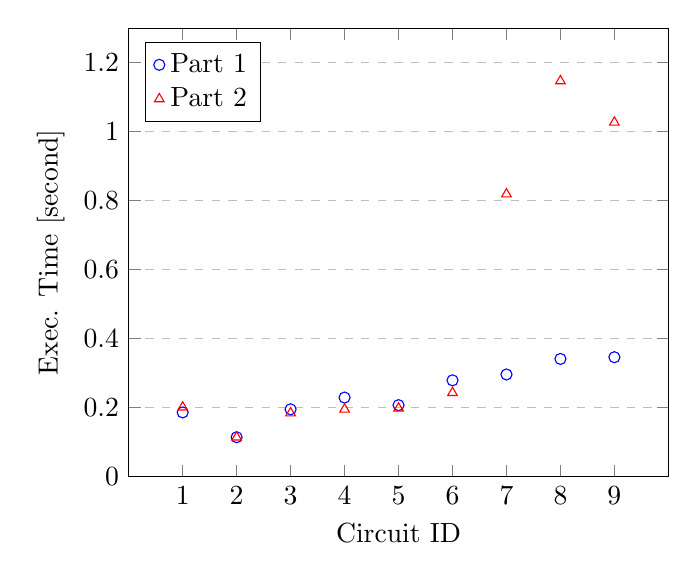
\begin{tikzpicture}
\begin{axis}[
    xlabel={Circuit ID},
    ylabel={Exec. Time [second]},
    xmin=0, xmax=10,
    ymin=0, ymax=1.3,
    xtick={1,2,3,4,5,6,7,8,9},
    ytick={0,0.2,0.4,0.6,0.8,1,1.2},
    legend pos=north west,
    ymajorgrids=true,
    grid style=dashed,
    only marks,
]

\addplot[
    color=blue,
    mark=o,
    ]
    coordinates {
    (1,0.186)(2,0.114)(3,0.195)(4,0.229)(5,0.207)(6,0.279)(7,0.296)(8,0.341)(9,0.346)
    };
    \addlegendentry{Part 1}
    
\addplot[
    color=red,
    mark=triangle,
    ]
    coordinates {
    (1,0.201)(2,0.114)(3,0.184)(4,0.195)(5,0.198)(6,0.243)(7,0.819)(8,1.147)(9,1.027)
    };
    \addlegendentry{Part 2}
    
\end{axis}
\end{tikzpicture}
\caption{Plot of mean execution time for each circuit}
\label{plot}
\end{figure}

From Figure \ref{plot}, we observe that for Part 1, the most determinant factors seem to be the number of peers and operations, even though it also seems correlated with the appearance of multiplication gates in the circuit. With only 3 peers and 5 gates (with 3 multiplication), circuit 7 is close to circuit 6 that has 4 peers and 3 gates (and 0 multiplication). This is justified by the fact that the generation of Beaver triplets requires additional computation, scaled to the number of multiplication gates and the gate itself requires additional message passing. Nevertheless, for Part 1, the impact remains low.\\
When comparing with Part 2 however, the presence of multiplication gate in a circuit has a much bigger impact. Indeed, from circuit 1 to circuit 6, the execution times for both Parts are almost identical. From circuit 7 to circuit 9, the execution times increase drastically and from the comparison with Part 1 for the same circuits, we know this is due to the presence of multiplication gates since the implementations of those Parts are very similar except when those gates are involved (all pre-processing for beaver triples is done only if the number of multiplication gate is greater than zero). This is not a surprise since the BFV beaver generation requires the creation of an additional dedicated network, which has a small waiting time for all parties to connect. \\

Taking this additional waiting time for connections into account, we note Circuit 8 has the largest difference of time to complete from Part I, which is largely due to the fact that it has the most parties between all the circuits and thus requires more message passing. In particular, for an initial Beaver generation protocol with \mathcal{N} parties, an additional new party adds \mathcal{4N} new messages to the network.

\section{Discussion}
\begin{itemize}
    \item As we saw, the loss of the assumption of the trusted party reduces greatly the computational speed. Nevertheless, Part 2 demonstrates the feasibility of having a secure multiparty computation without a trusted third party. In addition, Part 2 shows how \textbf{BFV} simulates an ideal execution which has a trusted third party and thus we can conclude that the \textbf{BFV} protocol is secure.\\
    \item With respecting the initial goal of the \textbf{SMC}, the first model cannot guarantee security in an environment which does not provide a trusted third party, thus in such environment, only the second model can guarantee privacy for the parties exchanging messages.\\
    \item When a trusted third party is available the first model seems to be more appropriate, due to its' better scaling when the number of parties or the number of multiplication gates grows large. We cannot however forget that such trusted third party falls under an "ideal world" scenario.\\
    \item We could imagine a new age notary that is responsible to act as a trusted third party in remote and digital transactions. Suppose multiple large private companies want to invest in a single project together. They all have a certain amount of money to invest in it but do not wish to reveal to the other companies that amount since it could reveal information on the companies' equity and reinvestment ratio. The notary could act as a trusted third party between the multiple private organizations to compute the total potential initial investment of the project.\\
    
    \item Of course, such notary not only might not be entirely trusted and could corrupt the whole computation but has a certain price. Since the second model simulates the first model, the companies could use \textbf{BFV} instead and use the money needed for the notary to increase the project size. \\
    
    \item The use of homomorphic encryption has extremely high potential in financial valuation in general. When previously private companies would hide most of their information and most valuations of their stock values were based on very vast assumptions, homomorphic encryption could bring a new age to evaluating private company stock values while keeping them entirely private. 
\end{itemize}

\section{Conclusion}
\begin{itemize}
    In conclusion, we learned to use the Go language and deepened our understanding of the SMC protocol and homomorphic encryption (especially the BFV scheme), while applying our theoretical knowledge to a concrete project. We also saw how to do a proper performance evaluation and comparison between two distinct implementations. Finally, we learned to work in a team in a unique context, where it is impossible to discuss and work in the same room about an ongoing project.
\end{itemize}

\bibliographystyle{IEEEtran}
\bibliography{bib}
\end{document}
